\frontmatter

%! An dieser Stelle eingeben, welche Ditelseite verwendet wird!
%Titelseite

\begin{titlepage}
\begin{center}

\textbf{\Huge Projektarbeit}\\
\vspace{1.5cm}
\LARGE{\titel \\}
\vspace{1.5cm}
\end{center}
\begin{flushleft}
\large{
\begin{tabular}{l l r}
\vspace{1.0cm}
\textbf{Vorgelegt am:}\quad\quad\quad & \abgabedatum\\

\textbf{Von:}           ~ & \textbf{\autoreins}\\
                        ~ & \textbf{\autorzwei}\\
\vspace{1.0cm}
                        ~ & \textbf{\autordrei}\\

\textbf{Studiengang:}   ~ & \studiengang \\
\vspace{1.0cm}
\textbf{Studienrichtung:} ~ & \studienrichtung \\
\vspace{1.0cm}
\textbf{Seminargruppe:} ~ & \seminargruppe \\

\textbf{Matrikelnummer:} ~ & \matnumeins \\
                         ~ & \matnumzwei \\
\vspace{1.0cm}
                         ~ & \matnumdrei \\
\textbf{Gutachter:}     ~ & \betreuereins \\ ~ & (\institutioneins)\\
                        ~ & \betreuerzwei \\ ~ & (\institutionzwei)\\

\end{tabular}}
\end{flushleft}
\end{titlepage}
\newpage

%\newpage 
%\thispagestyle{empty}
%\quad  \addtocounter{page}{-1}
%\newpage

%? Inhaltsverzeichnis
\tableofcontents
\newpage

%? Abbildungsverzeichnis
\listoffigures
\newpage

%? Tabellenverzeichnis
\listoftables
\newpage

%? Abkürzungsverzeichnis
\include{inhalt/Abkürzungen}


%! Ab hier der Hauptteil, hier werden alle Kapitel eingetragen, die zur Arbeit gehören!
\mainmatter

%Alle Seiten beginnen mit der Oberüberschrift
\section{Einleitung}
Die ist eine PDF mit der Vorlage erstellt, um die Funktion und Formatierung dieser zu zeigen.
Deswegen wird in dieser Seite direkt ein Zitat\onlinezitat{LogikSim} verwendet.

\absatz Ganz wichtig zu wissen ist, dass \ac*{SSH} eine Abkürzung ist.

\absatz Ein Bild sollte außerdem nicht fehlen.
\bild[1.0]{schaltung1.png}{Ich bin ein tolles Bild}
\Blinddocument
%Kapitel groß endet mit:
\newpage
\section{Kapitel 2}
\subsection{Kapitel 2.1}

\newpage
\section{Kapitel 3
}

%Beispiel für eine Abbildung
\begin{figure}[H]
    \centering
    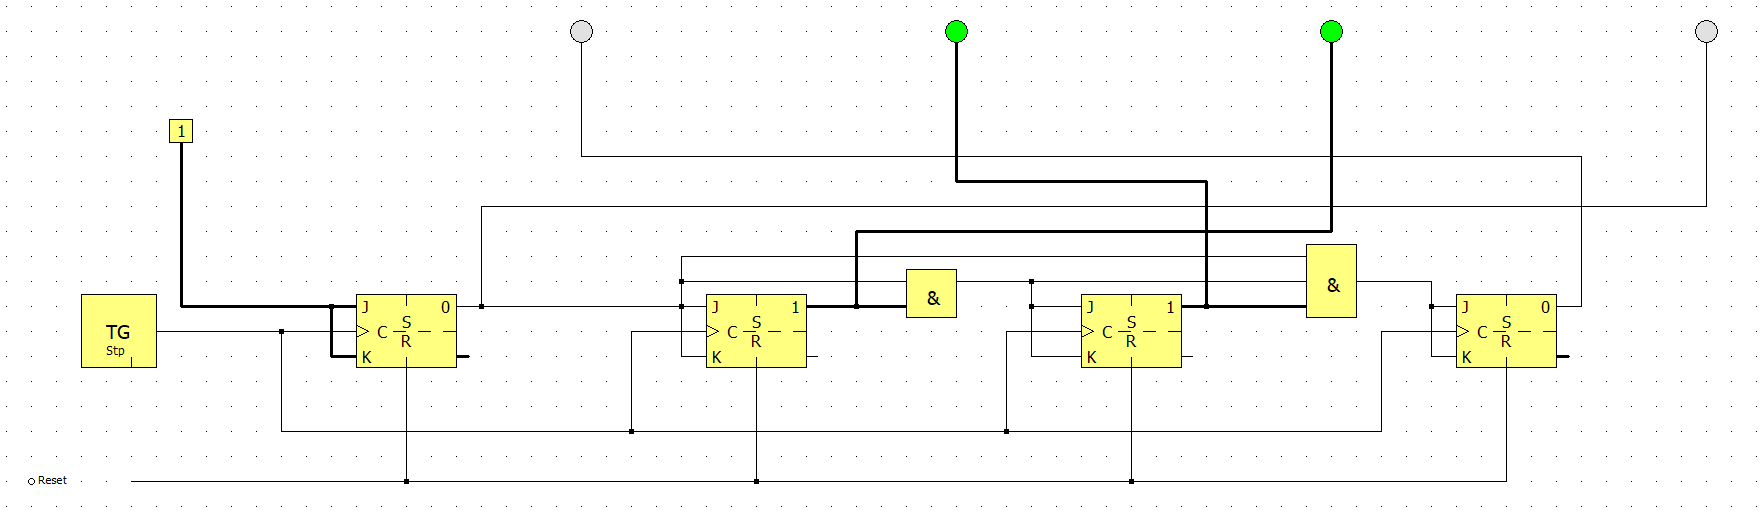
\includegraphics[width=1.0\columnwidth]{bilder/schaltung1.png}
    \caption{4-Bit synchroner Vorwärtszähler}
    \label{fig:4-Bit synchroner Vorwärtszähler}
\end{figure}


\newpage
\section{Kapitel 4}
\subsection{Kapitel 4.1}

\subsection{Kapitel 4.2}

\subsection{Kapitel 4.3}
\newpage
\section{Fazit}


\newpage

%! Ab hier der Schlussteil
%Überschrift Anhang fehlt noch.

%? Quellen und Literaturverzeichnis
%Literaturverzeichnis muss noch formatiert werden
\printbibliography

%? Anhang
%!	Anhang

\clearpage
\appendix
\clearpage

%! Section Befehl wird umgeschrieben, damit keine Überschriften mehr angezeigt werden
%!Kann falls Überschriften gewollt sind entfern werden oder erst später eingefügt
% Beginn 
\renewcommand{\section}[1]{
\par\refstepcounter{section}
\sectionmark{#1}
\addcontentsline{atoc}{section}{\protect\numberline{\thesection}#1}
\lohead{\textnormal{#1}}
} % Ende

%! Hier kann man sich anpassen, wie Abbildungen im Anhang dargestellt werden.
%! Bitte eins der beiden Auskommentieren
%? Möglichkeit 1 ohne Nummerierung und ohne Abbildung davor 
%\renewcommand{\bild}[3][1.0]{\begin{figure}[H]
%	\centering
%	\includegraphics[width=#1\columnwidth]{bilder/#2}
%	\caption*{#3}
%	\label{fig:#3}
%	\end{figure}}

%? Möglichkeit 2 mit Nummerierung und Abbildung, aber nicht im Abbildungsverzeichnis
\renewcommand{\bild}[3][1.0]{\begin{figure}[H]
	\centering
	\includegraphics[width=#1\columnwidth]{bilder/#2}
	\caption[]{#3}
	\label{fig:#3}
	\end{figure}}

%! Anhang 1
\section{Erster toller Anhang}
Hihi hier kommt eigentlich ein Anhangverzeichnis hin :D
\clearpage

%! Anhang 2
\section{Inhalt der CD}
CD mit folgenden Inhalten:
\begin{itemize}
	\item dieses Dokument
	\item Latex Dateien
	\item Youtube-Video als Bonus
\end{itemize}
 \clearpage

%! Eidestattliche Erklärung, hier zwischen Version für einen oder mehrere Autoren umschalten
\input{inhalt/Erklärung_Praxisbeleg}
%\input{inhalt/Erklärung_3Autoren}

\pagenumbering{gobble}

%? Eidestattliche Erklärung
\include{inhalt/Erklärung}